\chapter{Improving processor performance}
The performance of a processor is defined by the the time it takes to execute a program. This time span, called \emph{CPU time}, can be expressed as:

\begin{equation*}
  \text{CPU time} = \frac{\text{Seconds}}{\text{Program}} = \frac{\text{Clock cycles}}{\text{Program}} \cdot T_{ck}
\end{equation*}
where $T_{ck}$ is the clock period.

The first term can be decomposed further by computing the total number of instructions inside a program, called \emph{instruction count} (IC), which is known given the assembly code of the program. From this figure and the total number of clock cycles, the average number of \emph{clock cycles per instruction} (CPI)\footnote{Sometimes, also the inverse figure can be used, that is \emph{instructions per clock} (IPC).} can be derived. By factoring in these quantities, the final expression of CPU time is as follows \cite[p.~53]{hennessy17}:

\begin{equation}\label{eq:perf}
  \text{CPU time} = \text{IC} \cdot \text{CPI} \cdot T_{ck} 
\end{equation}

Equation \eqref{eq:perf} shows that the processor performance is directly and equally dependent on three factors:
\begin{itemize}
  \item Clock period, which depends mainly on the implementation technology and the microarchitectural choices (e.g. pipeline depth).
  \item Instruction count, which is determined for the most part by the ISA (see section \ref{sec:isas}) and compiler technology.
  \item CPI, which is dependant on both the ISA and the architecture.
\end{itemize}
The goal is then to minimize each of these terms, but it is evident that none of these parameters can be modified without affecting the others, as many design choices influence many of them.

\section{Instruction-level parallelism}
Earliest processors executed instructions one at a time, fetching a new one only after the previous has finished, leading to a number of clock cycles per instruction greater than one, and in particular equal to the number of stages an instruction must get through. This processor, where $\text{CPI} > 1$, are called \emph{subscalar}. To illustrate the situation, in the example of the classic 5-stage RISC pipeline (fetch, decode, execute, memory access, write back), a subscalar processor would execute three consecutive instructions as shown in figure \ref{fig:subscalar}, taking a total of 15 clock cycles.

\begin{figure}[hbtp]
  \centering
  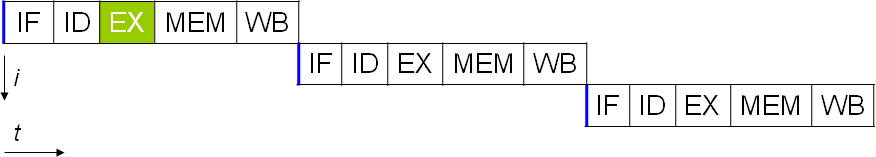
\includegraphics[width=0.8\textwidth]{img/subscalar.png}
  \caption{Subscalar processor}
  \label{fig:subscalar}
\end{figure}

Starting from the mid 80s, processor architects introduced \emph{pipelining} to improve performance by overlapping the execution of different instructions. This overlap means that at any given point in time there can be multiple instructions running in different stages of the processor, that is \emph{in parallel}, hence the term \emph{instruction-level parallelism} (ILP), which is a fundamental concept in developing techniques to enhance processor performance. For the same example of figure \ref{fig:subscalar}, a pipelined processor could theoretically achieve a CPI of 1, executing one instruction for each clock cycle (see figure \ref{fig:scalar}). Processors of this kind are called \emph{scalar}.

\begin{figure}[hbtp]
  \centering
  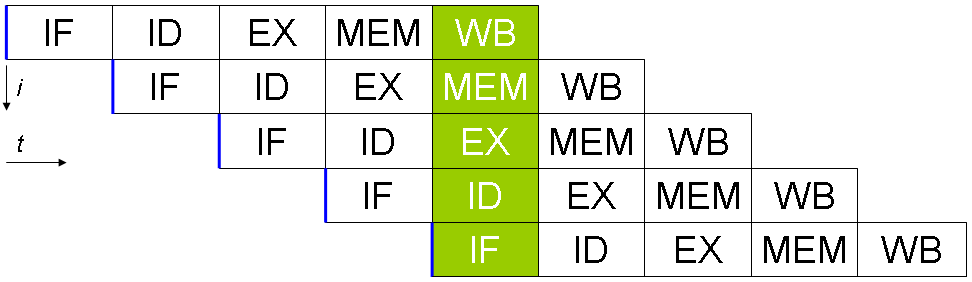
\includegraphics[width=0.8\textwidth]{img/scalar.png}
  \caption{Scalar processor}
  \label{fig:scalar}
\end{figure}

In practice however, data and control dependencies between successive instructions could cause hazards and force the pipeline to stall, causing CPI to rise once again at values greater than one. Those hazards become more likely and more expensive to manage the more pipeline stages are introduced and that is a clear example of a tradeoff between two factors of the performance equation \eqref{eq:perf}, as a deeper pipeline shortens the critical path and thus reduces the clock period, but at the same time increases the CPI. That is the reason why designers at some point had to find other architectural solutions to improve performance.


\section{Beyond static scheduling}

\section{Speculation}

